\documentclass[review]{elsarticle}

\usepackage{lineno,hyperref}

\usepackage{graphicx}
\usepackage[table]{xcolor}
\usepackage{booktabs}


\modulolinenumbers[5]

% \journal{Journal of \LaTeX\ Templates}


%% `Elsevier LaTeX' style
\bibliographystyle{elsarticle-num}
%%%%%%%%%%%%%%%%%%%%%%%

\begin{document}

\begin{frontmatter}

\title{Parallel Algorithms for Kernel Density Estimation}


%% or include affiliations in footnotes:
\author[oden]{Namo Wichitrnithed}
\ead{namo@utexas.edu}

\author[oden]{Rylan Spence}
\ead{rylan.spence@utexas.edu}

\affiliation[oden]{organization={Oden Institute for Computational Engineering and Sciences, University of Texas at Austin},
            city={Austin},
            postcode={78712},
            state={TX},
            country={USA}}


\begin{abstract}

\end{abstract}

\begin{keyword}
Kernel Density Estimation \sep Parallel computing \sep Cuda
\end{keyword}

\end{frontmatter}


\section{Introduction}

\begin{itemize}
    \item \textbf{Project Motivation}
    \item \textbf{Brief literary review KDE (See References Below)}
    \item \textbf{Brief literary review Parallized KDE (See References Below)}
\end{itemize}

\section{Multi-Core Programming Models}

\begin{itemize}
    \item \textbf{MPI} \newline
    Basic Review of MPI Architecture
    \item \textbf{GPU} \newline
    Basic Review of GPU Architecture
\end{itemize}

\section{Serial vs.Vectorized vs. Multi-Core Kernel Density Estimation}

\begin{itemize}
    \item \textbf{Serial Algorithm Pseudo Code}
    \item \textbf{SIMD Algorithm Pseudo Code}
    \item \textbf{MPI Algorithm Pseudo Code}
    \item \textbf{Cuda Algorithm Pseudo Code} \newline
    \item 
    \begin{figure}
      \centering
      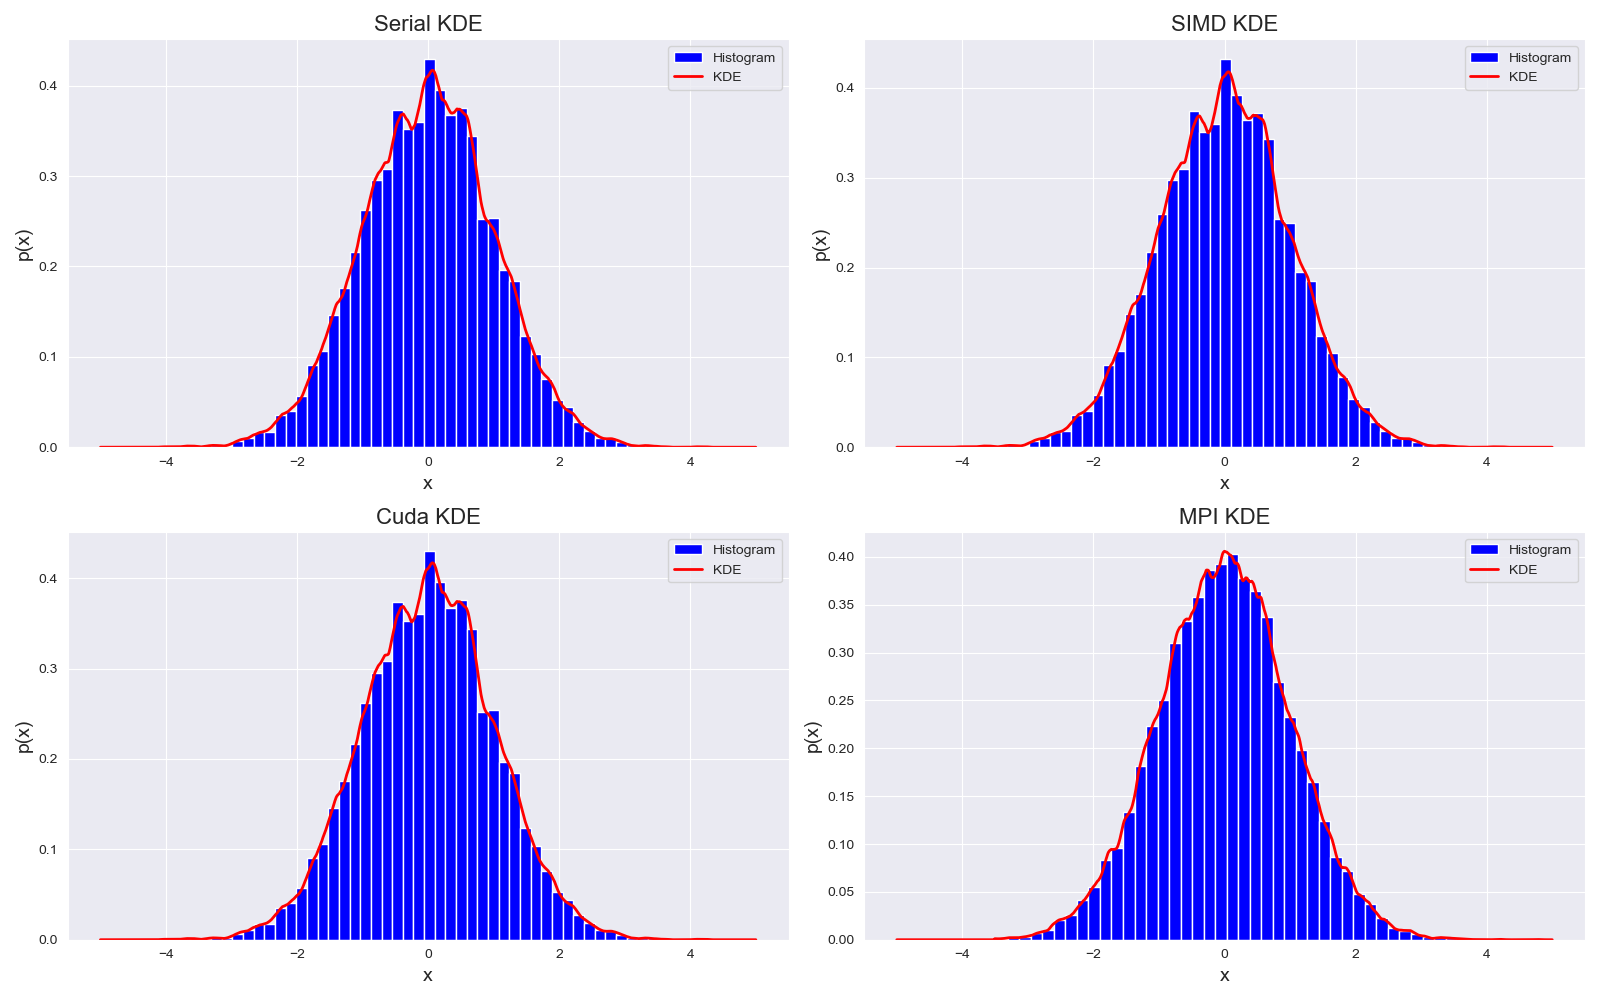
\includegraphics[width=15cm,height=12cm]{figures/multiple_kde_temp.png}
      \caption{Kernel Density Estimates for all four proposed algorithms}
      \label{fig:multiple_kde}
    \end{figure}
\end{itemize}


\section{Results}

\subsection{Quantititative Comparison}
\begin{figure}
  \centering
  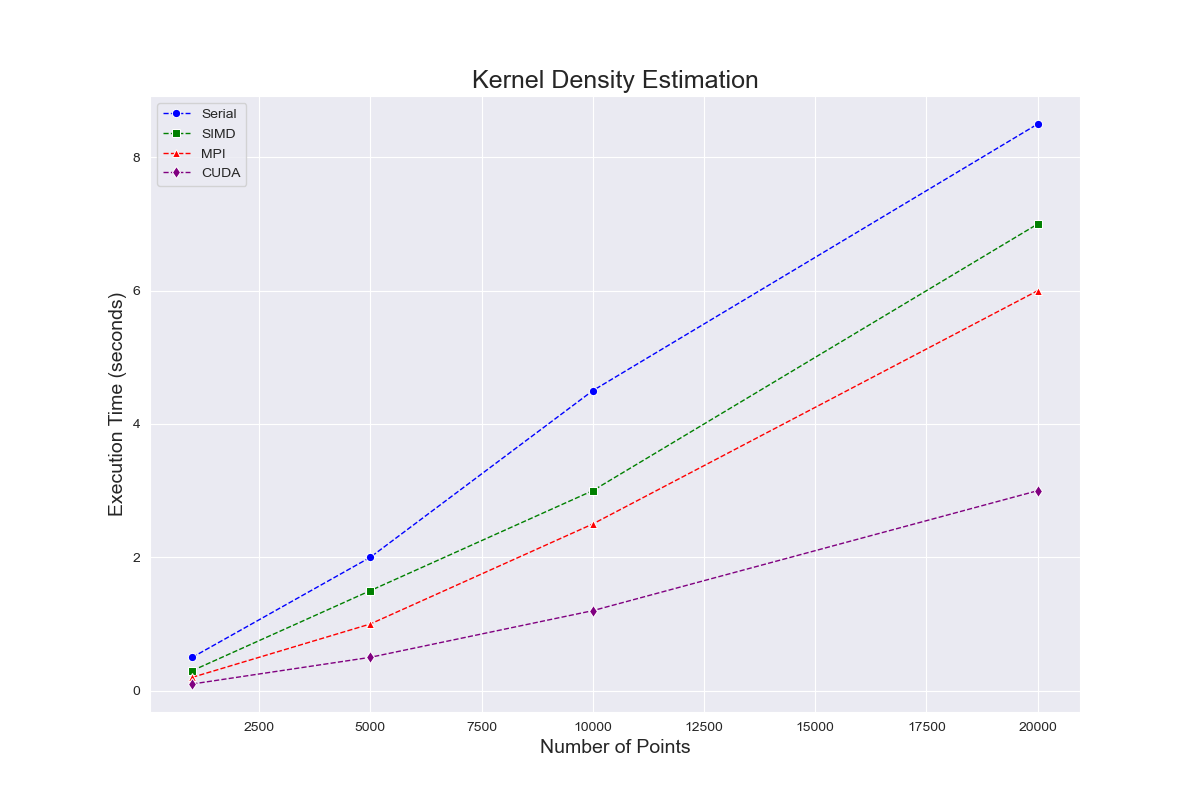
\includegraphics[width=15cm,height=12cm]{figures/execution_time_npoints_temp.png}
  \caption{Execution times (in secs) of a kernel estimation  as a function of the grid points. }
  \label{fig:time_npoints}
\end{figure}

\begin{figure}
  \centering
  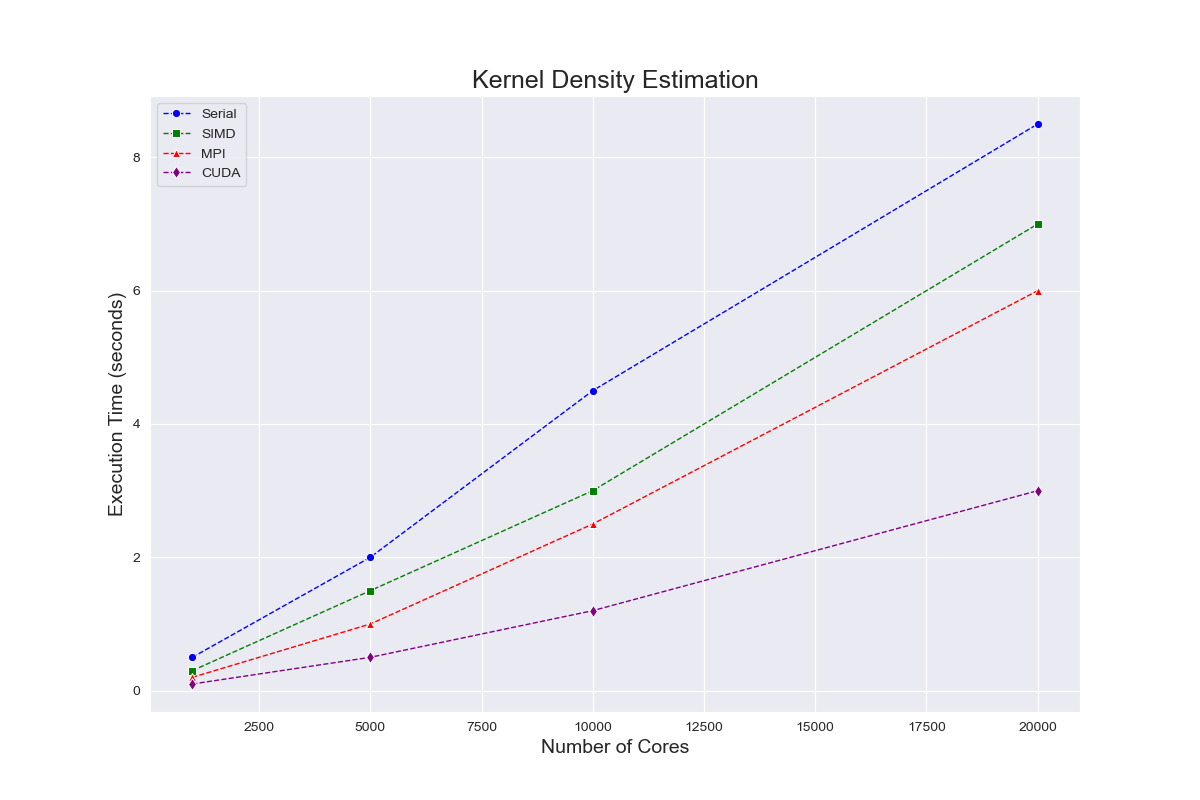
\includegraphics[width=15cm,height=12cm]{figures/execution_time_ncores_temp.png}
  \caption{Execution times (in secs) of a kernel estimation  as a function of the number of cores.}
  \label{fig:time_ncores}
\end{figure}

\begin{figure}
  \centering
  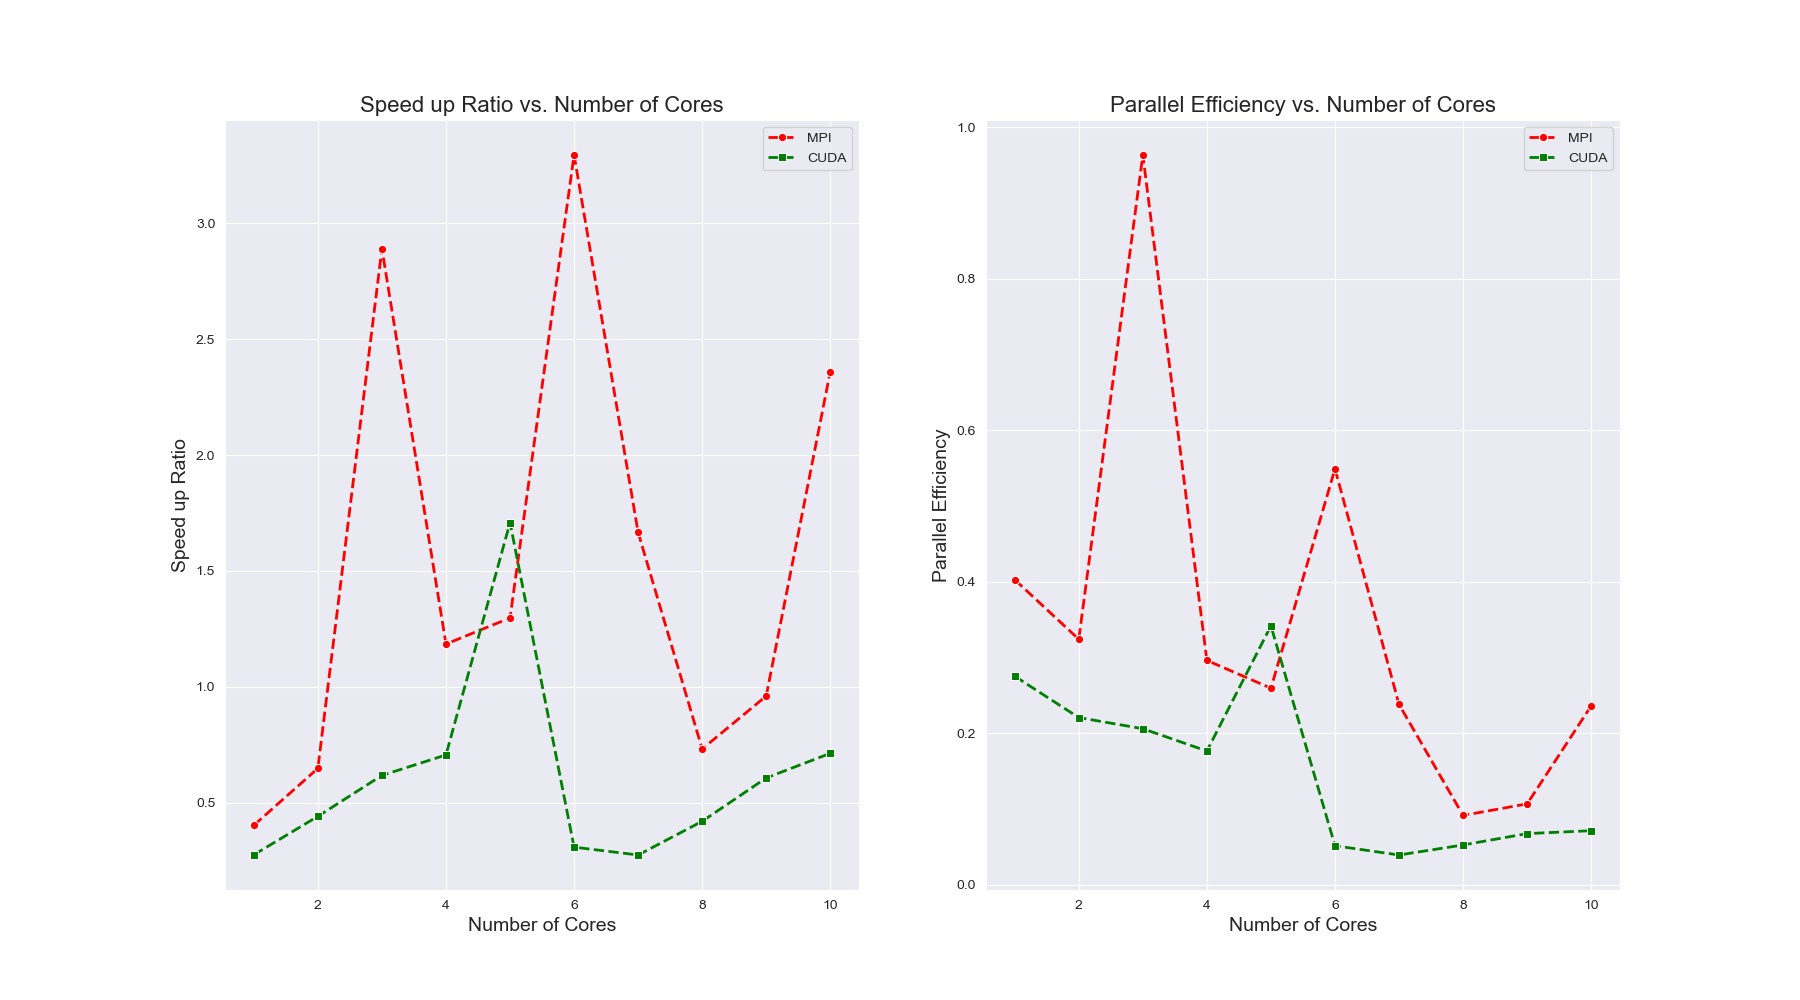
\includegraphics[scale=0.35]{figures/speedup_efficiency.png}
  \caption{Performance of the MPI-parallel algorithm for  KDE on the test data set (n = ?, m = ?): (a) speed up ratio and (b) parallel efficiency - defined as speedup ratio divided by number of CPU cores.}
  \label{fig:time_ncores}
\end{figure}


\subsection{Qualitative Comparison}

\begin{table}[h]
  \centering
\begin{tabular}{l *5c @{}}    \toprule
  Kernel Density Algorithm & \emph{Serial} & \emph{SIMD}  & \emph{MPI}  & \emph{Cuda}  \\\midrule
\rowcolor{blue!35} Lines of code & 12 & 17 & 10 & 12  \\ \bottomrule
 \hline
\end{tabular}
\caption{Lines of code in Programming Models}
\label{tab:sim_attr}
\end{table}


\section{Conclusions}

% \section*{References}

\nocite{*}
\bibliography{mybibfile}

\end{document}